\section{Preamplifier}

The photocurrents created by our detector are in the range of microampere where they are vulnerable to noise.
Using a preamplifier, we can increase the amplitude of the signal for an improved signal-to-noise ratio.
The typical photocurrent preamplifier is based on the transimpedance (current-to-voltage) amplifier design using a voltage-feedback operational amplifier.
Converting the current to a voltage signal has the benefit that the voltage signal can be easily visualized with an oscilloscope.
Furthermore, the voltage-feedback operational amplifier design appears to be more common than the current-feedback operational amplifier, as manufacturers offer much more choice and they are more prominent in the literature.
That said, current-feedback operational amplifiers are reported to be a viable solution for high-speed and high-bandwidth applications, see Ref.~\cite[p.~110]{Jung05} for an overview of the benefits of current-feedback amplifiers and Ref.~\cite[Ch.~9]{Carter17} for a comparison with voltage-feedback amplifiers.

In the following, we will always refer to the voltage-feedback operational amplifier if not noted otherwise.
Moreover, we expect the reader to be familiar with the foundations of the operational amplifier.
Well-written introductions to this topic can be found in \cite[Ch.~1]{Jung05} and \cite[Ch.~3]{Carter17}.

\subsection{Basic design}

The basic design of a transimpedance amplifier is illustrated in~\Cref{fig:basic_transimpedance}.
Ignoring imperfections of the photodiode, we can represent the photodiode as a current source.
The non-inverting input of the operational amplifier is connected to ground.
The inverting input is coupled with the output of the operational amplifier via a feedback impedance $Z_f$.
\begin{figure}[H]
	\centering
	\begin{circuitikz}
		\draw (0, 0) node[op amp](opamp){};
		\draw (opamp.+) -- +(0, -1) node[ground](gnd1){};
		\draw (opamp.out) -- +(1, 0) node[ocirc, label=$V_\text{out}$]{};
		\draw (opamp.-) node[circ]{} -- +(-2, 0) node(node1){} to[current source, invert, l=$I_\text{in}$] (node1 |- gnd1) node[ground]{};
		\draw (opamp.-) |- (-1, 2) to[generic, l=$Z_f$] (1,2) -| (opamp.out);
	\end{circuitikz}
	\caption{Basic transimpedance amplifier using voltage feedback operational amplifier.}\label{fig:basic_transimpedance}
\end{figure}
The ideal operation amplifier has zero input current, thus, in the node of the inverting input of the operational amplifier Kirchhoff's law states that the current going through the feedback impedance has to cancel the current of the current source $I_\text{in}$.
The current through the feedback impedance $Z_f$ can be expressed in terms of the feedback impedance $Z_f$ and the output voltage $V_\text{out}$ of the operational amplifier through the use of Ohm's law, yielding,
\begin{equation}
	V_\text{out}=-Z_fI_\text{in}
	\label{eq:transimpedance}.
\end{equation}
Given a maximum current $I_\text{in}$ and a desired maximum output voltage $V_\text{out}$, \Cref{eq:transimpedance} determines the feedback impedance.
Limitations arise for real operational amplifiers where the output voltage is limited to be below the supply voltage of the operational amplifier.


Aside from photodiode applications, it is more common to find the inverting (voltage-to-voltage) operational amplifier in the literature.
By using the source transformation on the current source with a parallel impedance in the transimpedance amplifier circuit, we can recover the inverting operational amplifier circuit, and thereby easily use results obtained for the inverting amplifier design.
\begin{figure}[H]
	\begin{subfigure}[t]{.5\textwidth}
		\centering
		\begin{circuitikz}
			\draw (0, 0) node[op amp](opamp){};
			\draw (opamp.+) -- +(0, -1) node[ground](gnd1){};
			\draw (opamp.out) -- +(1, 0) node[ocirc, label=$V_\text{out}$]{};
			\draw (opamp.-) node[circ]{} -- +(-3, 0) node(node1){} to[current source, invert, l=$I_\text{in}$] (node1 |- gnd1) node[ground]{};
			\draw (opamp.-) node[circ]{} -- +(-1.5, 0) node(node1){} to[generic, invert, l=$Z_\text{in}$] (node1 |- gnd1) node[ground]{};
			\draw (opamp.-) |- (-1, 2) to[generic, l=$Z_f$] (1,2) -| (opamp.out);
		\end{circuitikz}
		\caption{Transimpedance amplifier.}
	\end{subfigure}
	\begin{subfigure}[t]{.5\textwidth}
		\centering
		\begin{circuitikz}
			\draw (0, 0) node[op amp](opamp){};
			\draw (opamp.+) -- +(0, -1) node[ground](gnd1){};
			\draw (opamp.out) -- +(1, 0) node[ocirc, label=$V_\text{out}$]{};
			\draw (opamp.-) node[circ]{} to[generic, invert, l_=$Z_\text{in}$] +(-3, 0) node(node1){} to[voltage source, l=$V_\text{in}{=}Z_\text{in}I_\text{in}$] (node1 |- gnd1) node[ground]{};
			\draw (opamp.-) |- (-1, 2) to[generic, l=$Z_f$] (1,2) -| (opamp.out);
		\end{circuitikz}
		\caption{Inverting amplifier.}
	\end{subfigure}
	\caption{Equivalence between transimpedance and inverting amplifier using source transformation.}\label{fig:equivalence_transimpedance_inverting}
\end{figure}
\Cref{fig:equivalence_transimpedance_inverting} shows the source transformation applied to transimpedance and inverting amplifier circuits.
Given a current source $I_\text{in}$ with parallel impedance $Z_\text{in}$ the equivalent voltage source has value $V_\text{in}=Z_\text{in}I_\text{in}$ with impedance $Z_\text{in}$ in series.

\subsection{Input offset voltage}

Real operational amplifiers only reduce the voltage difference between the inverting and non-inverting input to a non-zero input offset voltage.
For high-precision operational amplifiers, the input offset voltage is in the range of microvolts.
We can model the input offset voltage as a voltage source at the non-inverting input of an ideal operational amplifier in our transimpedance circuit, as can be seen from \Cref{fig:input_offset_voltage_transimpedance}.
In \Cref{fig:input_offset_voltage_transimpedance} we amended the basic transimpedance circuit of \Cref{fig:basic_transimpedance} by inserting a voltage source with the input offset voltage between the non-inverting input and ground.
\begin{figure}[H]
	\centering
	\begin{circuitikz}
		\draw (0, 0) node[op amp](opamp){};
		\draw (opamp.-) |- (-1, 2) to[generic, l=$Z_f$] (1,2) -| (opamp.out);
		\draw (opamp.out) -- +(1, 0) node[ocirc, label=$V_\text{out}$]{};
		\draw (opamp.+) -- ++(0, -.5) node(node1){} to[voltage source, l=$V_\text{offset}$] ++(0, -2) node[ground](gnd1){};
		\draw (opamp.-) node[circ]{} -- +(-2, 0) node(node2){} -- (node2 |- node1) to[current source, invert, l=$I_\text{in}$] (node2 |- gnd1) node[ground]{};
	\end{circuitikz}
	\caption{Input offset voltage in the transimpedance amplifier.}\label{fig:input_offset_voltage_transimpedance}
\end{figure}
In order to estimate the output offset $V_\text{out}$ caused by the input offset voltage $V_\text{offset}$ we adapt the picture of the inverting amplifier.
\Cref{fig:input_offset_voltage_inverting} shows an inverting amplifier circuit with input impedance $Z_\text{in}$ and input offset voltage $V_\text{offset}$ at the non-inverting input of the operational amplifier.
According to the superposition theorem, we can replace the input voltage source with a short circuit to estimate the contribution of the input offset voltage source.
\begin{figure}[H]
	\centering
	\begin{circuitikz}
		\draw (0, 0) node[op amp](opamp){};
		\draw (opamp.-) |- (-1, 2) to[generic, l=$Z_f$] (1,2) -| (opamp.out);
		\draw (opamp.out) -- +(1, 0) node[ocirc, label=$V_\text{out}$]{};
		\draw (opamp.+) -- ++(0, -.5) node(node1){} to[voltage source, l=$V_\text{offset}$] ++(0, -2) node[ground](gnd1){};
		\draw (opamp.-) node[circ]{} -- +(-2, 0) node(node2){} -- (node2 |- node1) to[generic, l=$Z_\text{in}$] (node2 |- gnd1) node[ground]{};
	\end{circuitikz}
	\caption{Input offset voltage in the inverting amplifier.}\label{fig:input_offset_voltage_inverting}
\end{figure}
From \Cref{fig:input_offset_voltage_inverting} we identify input and feedback impedance as a voltage divider in which the input and output nodes are exchanged.
The respective transfer function reads,
\begin{equation}
	V_\text{out}=-\frac{R_f+R_\text{in}}{R_\text{in}}V_\text{offset}=-\left(1+\frac{R_f}{R_\text{in}}\right)V_\text{offset}
	\label{eq:input_offset_voltage}.
\end{equation}
Comparing \Cref{eq:input_offset_voltage} with \Cref{eq:transimpedance} discloses a difference in gain.
The gain of the input signal in Eq. 1 is commonly referred to as signal gain. 
The gain of a signal applied directly to the inputs of the operational amplifier is referred to as noise gain.
In the case of the position-sensitive detector, the input resistance is of order \SI{10}{\kilo\ohm}.
Using a feedback resistance of $R_f=\SI{100}{\kilo\ohm}$ we find that the input offset voltage experiences a gain of 11.

One approach to compensate for the input offset voltage as described is depicted in \Cref{fig:input_offset_voltage_compensation}, see also Ref~\cite[p.~54]{Jung05}.
A potentiometer with maximum resistance Rp connects the positive and negative supply voltage.
The wiper of the potentiometer is connected with a first resistor R1 to a node.
The node is connected with a second resistor R2 and an optional bypass capacitor to ground.
Finally, the equivalent input offset voltage source connects the node with the non-inverting input of the operational amplifier.
\begin{figure}[H]
	\centering
	\begin{circuitikz}
		\draw (0, 3) node[ocirc, label=$+V_\text{supply}$]{} to[potentiometer, n=poti, l_=$R_p$] ++(0, -3) node[ocirc, label=$-V_\text{supply}$, rotate=180]{};
		\draw (poti.wiper) to[resistor, l=$R_1$] ++(2, 0) node(node1)[circ]{} to[resistor, l=$R_2$] ++(0, -2) node(gnd)[ground]{};
		\draw (node1) to[voltage source, l_=$V_\text{offset}$, invert] ++(0, 2) node[ocirc, label=$V_+$]{};
		\draw (node1) -- ++(2, 0) to[capacitor, l=$C_1$] ++(0, -2) node[ground]{};
	\end{circuitikz}
	\caption{Input offset voltage compensation using adjustable potentiometer.}\label{fig:input_offset_voltage_compensation}
\end{figure}
Let $0\leq x\geq1$ be the position of the potentiometer.
For $x=1/2$ the resistance of the potentiometer is $R_p/2$ and there is no offset compensation.
For $x<1/2$ the input offset compensation is negative to compensate for a positive input offset voltage.
For $x>1/2$ the input offset compensation is positive to compensate for a negative input offset voltage.
The maximum input offset compensation is obtained for $x=0$ and $x=1$.
Using circuit analysis techniques, we obtain,
\begin{equation}
	V_c(x)=\frac{R_2(1-2x)}{R_1+R_2-R_p(1-x)x}V_\text{supply},
\end{equation}
as an analytical expression for the input offset voltage compensation measured between the node and ground.
The maximum absolute value of the compensation voltage follows to be,
\begin{equation}
	V_c(0)=V_c(1)=\pm\frac{R_2}{R_1+R_2}V_\text{supply}.
\end{equation}
Given a maximum input offset voltage of \SI{100}{\micro\volt} and a supply voltage of \SI{15}{\volt}, we find approximate resistor values $R_1=\SI{3}{\mega\ohm}$ and $R_2=\SI{2}{\ohm}$.
The resistor value of the potentiometer $R_p$ should be chosen sufficiently large such to limit the current.
For example, a potentiometer resistance of $R_p=\SI{15}{\kilo\ohm}$ would limit the current to \SI{2}{\milli\ampere} with a heat dissipation of \SI{60}{\milli\watt}.
In practice, one should aim for a slightly higher maximum compensation voltage in order to handle resistor mismatches.

That said, there are some practical arguments against the use of the described input offset voltage compensation.
The first argument is that the low resistance of $R_2$ acts as a dominant source for thermal current noise density of about \SI{100}{\pico\ampere\per\sqrt\hertz}.
As this current noise contributes to the input of the transimpedance amplifier it gets amplified by the feedback impedance $Z_f$, yielding up to \SI{110}{\micro\volt\per\sqrt\hertz} in voltage noise density, which --- depending on the bandwidth --- surpasses the actual input offset voltage to compensate.
The second argument is that high-precision potentiometers with large dynamic range get very large and difficult to accommodate on a printed circuit board.

\subsection{Input bias current}

In addition to the input offset voltage $V_\text{offset}$, there is a second effect that causes an offset in the output voltage $V_\text{out}$.
This second effect stems from the small amount of current that is drawn from the inputs of the operational amplifier.
We highlighted the input currents in \Cref{fig:input_bias_current} where they are represented by the current flows $i_+$ and $i_-$ directly pointing into the inputs of the operational amplifier in the transimpedance circuit.
\begin{figure}[H]
	\centering
	\begin{circuitikz}
		\draw (0, 0) node[op amp](opamp){};
		\draw (opamp.out) -- +(0.5, 0) node(node1)[circ]{} -- ++(1.5, 0) node[ocirc, label=$V_\text{out}$]{};
		\draw (opamp.-) to[short, i<_=$i_-$] ++(-1, 0) node(node1a)[circ]{} |- (-1.5, 2) to[generic, l=$Z_f$] (1.5, 2) -| (node1);
		\draw (opamp.+) to[short, i<_=$i_+$] ++(-1, 0) node(node1b){} -- ++(0, -1) node(gnd)[ground]{};
		\draw (node1a) -- ++(-1.5, 0) node(node2a){} to[current source, invert, l=$I_\text{in}$] (node2a |- gnd) node[ground]{};
	\end{circuitikz}
	\caption{Input bias current offset in the transimpedance amplifier.}\label{fig:input_bias_current}
\end{figure}
Input bias currents for high-precision operational amplifier are in the range of picoamperes.
These small currents are usually difficult to measure and may differ between inputs.
The datasheet of the operational amplifier, therefore, doesn't report the input bias current per terminal but the mean $I_\text{bias}$ and the difference between the input currents $I_\text{offset}$.
The relationship between the mean input bias current $I_\text{bias}$ and the input offset current $I_\text{offset}$ with respect to the actual input bias currents $i_+,i_-$ is given below.
\begin{align}
	i_+=I_\text{bias}+\frac{1}{2}I_\text{offset} &&
	I_\text{offset}=i_+-i_- \\
	i_-=I_\text{bias}-\frac{1}{2}I_\text{offset} &&
	I_\text{bias}=\frac{i_++i_-}{2}
\end{align}
According to Ref.~\cite[p.~57]{Jung05} and Ref.~\cite[p.~25]{Graeme96} the effect of the input bias currents $i_+,i_-$ on the output voltage $V_\text{out}$ can be compensated with an impedance $Z_c$ at the non-inverting input of the operational amplifier.
\Cref{fig:input_bias_current_compensation} illustrates the inverting amplifier configuration with such a compensation impedance $Z_c$.
\begin{figure}[H]
	\centering
	\begin{circuitikz}
		\draw (0, 0) node[op amp](opamp){};
		\draw (opamp.out) -- +(0.5, 0) node(node1)[circ]{} -- ++(1.5, 0) node[ocirc, label=$V_\text{out}$]{};
		\draw (opamp.-) to[short, i<_=$i_-$] ++(-1, 0) node(node1a)[circ]{} |- (-1.5, 2) to[generic, l=$Z_f$] (1.5, 2) -| (node1);
		\draw (opamp.+) to[short, i<_=$i_+$] ++(-1, 0) node(node1b){} to[generic, l=$Z_c$] ++(0, -2) node(gnd)[ground]{};
		\draw (node1a) -- ++(-1.5, 0) node(node2a){} -- (node1b -| node2a) to[generic, l=$Z_\text{in}$] (node2a |- gnd) node[ground]{};
	\end{circuitikz}
	\caption{Input current offset compensation.}\label{fig:input_bias_current_compensation}
\end{figure}
Following the argumentation from Ref.~\cite[p.~383]{Terrel96}, the input bias current at the inverting input of the operational amplifier $i_-$ develops a voltage of $Z_fi_-$ over the feedback impedance $Z_f$.
The input bias current at the non-inverting input $i_-$ develops the voltage $Z_ci_-$ over the compensation resistor $Z_c$.
The voltage $Z_ci_-$ propagates through the voltage divider comprising the feedback and input impedance analogue to the input offset voltage.
According to the superposition theorem, both of these contributions add and yield,
\begin{equation}
	V_\text{out}=i_+Z_c\left(1+\frac{Z_f}{Z_\text{in}}\right)-i_-Z_f
	\label{eq:input_bias_current},
\end{equation}
at the output voltage.
If $i_+\approx i_-$ we can choose,
\begin{equation}
	Z_c=\frac{Z_\text{in}}{Z_\text{in}+Z_f},
\end{equation}
 to compensate for the output voltage offset caused by the input bias currents.
The condition $i_+\approx i_-$ is usually satisfied if the input offset current $I_\text{offset}$ reported in the datasheet is less than the mean input bias current $I_\text{bias}$.
High-precision operational amplifier usually have compensated bias currents that do not satisfy this condition.
In this case, there is no generic formula for the value of the compensation impedance $Z_c$ in terms of input and feedback impedance and one needs to perform impedance matching on a per-device basis.

\subsection{Stability and bandwidth}

The outputs of the transimpedance and inverting amplifier designs have a phase shift of \SI{180}{\degree}.
If an additional phase shift of \SI{180}{\degree} accumulates because of the inherent bandwidth limitations of the operational amplifier and the gain is equal or greater than unity, the conditions for oscillations are met and the amplifier will become unstable, see Ref.~\cite[p.~395]{Terrel96}.
By artificially limiting the bandwidth with an additional frequency pole, we can flatten out the frequency response at high frequencies, and thereby stabilize the amplifier, see Ref.~\cite[p.~184]{Kay12}.

\Cref{fig:bode_gain} shows a Bode plot of the open-loop (black) and noise gain (red) of an operational amplifier.
The noise gain separates into a compensated (solid) and uncompensated (dotted) branch.
\begin{figure}[H]
	\centering
	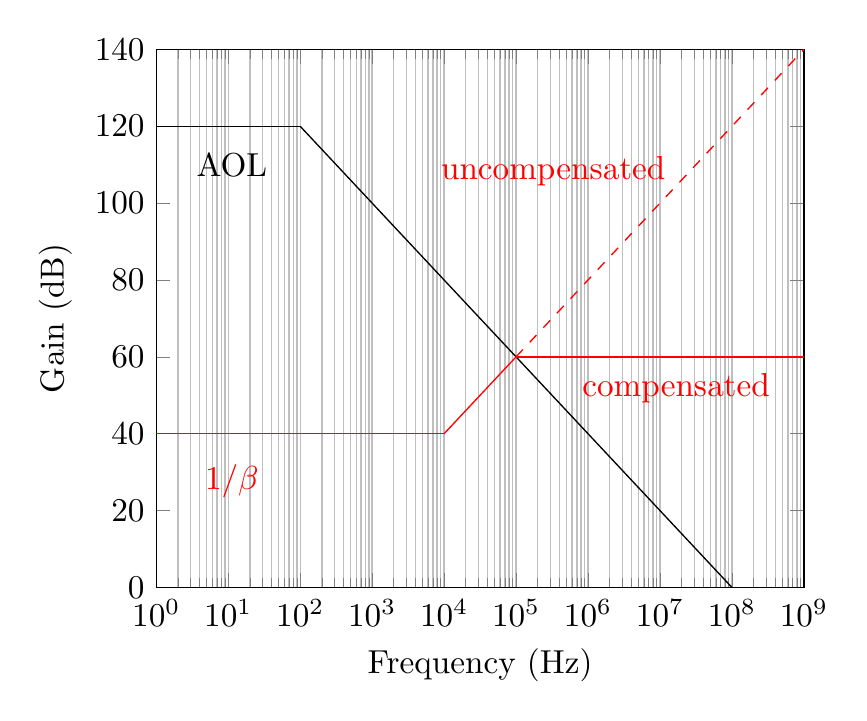
\begin{tikzpicture}[scale=1.2, transform shape]
		\begin{semilogxaxis}[xmin=1, xmax=1e9, xlabel=Frequency (Hz), ymin=0, ymax=140, ylabel=Gain (dB), ytick={0, 20, 40, 60, 80, 100, 120, 140}, grid=minor]
			\addplot[domain=1:1e2]{120};
			\addplot[domain=1e2:1e9]{160-20*log10(x)};
			\addplot[domain=1:1e4, color=red]{40};
			\addplot[domain=1e4:1e5, color=red]{-40+20*log10(x)};
			\addplot[domain=1e5:1e9, color=red]{60};
			\addplot[domain=1e5:1e9, dashed, color=red]{-40+20*log10(x)};
		\end{semilogxaxis}
		\node[label={AOL}] at (.8, 4.1) {};
		\node[label={[red]$1/\beta$}] at (.8, .7) {};
		\node[label={[red]compensated}] at (5.5, 1.7) {};
		\node[label={[red]uncompensated}] at (4.2, 4) {};
	\end{tikzpicture}
	\caption{Bode plot of the open-loop and closed-loop gain of the amplifier.}\label{fig:bode_gain}
\end{figure}
With the uncompensated branch we would observe instability due to oscillations.
The compensated branch is obtained through addition of a feedback capacitor.
According to Ref.~\cite[p.~113]{Jung05}, Ref.~\cite[p.~693]{Hobbs11} and Ref.~\cite[Ch.~3]{Graeme96} the value for the feedback capacitance is given by,
\begin{equation}
	C_f\geq\sqrt{\frac{C_\text{in}}{2\pi R_f f_u}}
	\label{eq:feedback_capacitance_approximation},
\end{equation}
wherein $R_f$ denotes the feedback resistance and $f_u$ the unity-gain-bandwidth of the operational amplifier.
The capacitance should be chosen larger to ensure design margin.
The unity-gain-bandwidth of the operational amplifier denotes the frequency where the open-loop gain equals unity and is reported in the datasheet as \gls{gbp} of the operational amplifier.
$C_\text{in}$ in \Cref{eq:feedback_capacitance_approximation} represents the sum of the input capacities of the amplifier circuit and the capacitance of the signal source.
According to Ref.~\cite[p.~185]{Carter17} a more exact formula for the feedback capacitance is given by,
\begin{align}
	C_f\geq\frac{C_\text{aux}}{2}\left(1+\sqrt{1+\frac{4C_\text{in}}{C_\text{aux}}}\right) &&
	C_\text{aux}=\frac{1}{2\pi R_f f_u}
	\label{eq:feedback_capacitance_exact},
\end{align}
which is also valid if not $C_\text{in}\gg C_f$.

\Cref{fig:capacitive_transimpedance} illustrates the transimpedance amplifier with capacitive elements.
Parallel to the current source $I_\text{in}$ we find the input capacitance $C_\text{in}$ comprising source capacitance and operational amplifier capacitance.
Parallel to the feedback resistance $R_f$ we find the feedback capacitance $C_f$ with value given in \Cref{eq:feedback_capacitance_exact} or \Cref{eq:feedback_capacitance_approximation}.
\begin{figure}[H]
	\centering
	\begin{circuitikz}
		\draw (0, 0) node[op amp](opamp){};
		\draw (opamp.+) -- +(0, -1) node[ground](gnd1){};
		\draw (opamp.out) -- +(1, 0) node[ocirc, label=$V_\text{out}$]{};
		\draw (opamp.-) node[circ]{} -- +(-4, 0) node(node1){} to[current source, invert, l=$I_\text{in}$] (node1 |- gnd1) node[ground]{};
		\draw (opamp.-) node[circ]{} -- +(-2, 0) node(node1){} to[capacitor, l=$C_\text{in}$] (node1 |- gnd1) node[ground]{};
		\draw (opamp.-) |- (-1, 2) to[resistor, l=$R_f$] (1, 2) -| (opamp.out);
		\draw (opamp.-) |- (-1, 3.5) to[capacitor, l=$C_f$] (1, 3.5) -| (opamp.out);
	\end{circuitikz}
	\caption{Transimpedance amplifier with capacitive elements.}\label{fig:capacitive_transimpedance}
\end{figure}
% TODO: why use noise gain
% TODO: definition open-loop gain, closed-loop gain
% TODO: why is rate of closure important for stability (relation with phase margin?)

As noted earlier, the bandwidth is reduced through the additional feedback capacitor.
The new bandwidth is now given by the RC pole formed by the feedback impedance,
\begin{equation}
	BW=\frac{1}{2\pi R_fC_f}.
\end{equation}
Given a unity-gain-bandwidth of the operational amplifier of $f_u=\SI{10}{\mega\hertz}$ and a feedback resistance of $R_f=\SI{100}{\kilo\ohm}$ \Cref{eq:feedback_capacitance_approximation} yields a minimum feedback capacitance of $C_f=\SI{4}{\pico\farad}$.
Together with $R_f$ this feedback capacitance limits the bandwidth to about \SI{400}{\kilo\hertz}.

\subsection{Noise density}

% TODO: (Jung, p. 80)
% TODO: thermal noise from resistor
% TODO: equivalent noise from operational amplifier